\chapter{Formulation}
The Arbitrary Lagrangian-Eulerian (ALE) Formulation is the modelling technique to couple/decouple the motion of particles or bodies in the Eulerian and Lagrangian Formulation. The formulation is commonly employed in Fluid-Structure Interaction Problems, where the domain of the solid is affected by the fluid and, the other way round \cite{ait2002}.
The key feature about ALE formulation is the decomposition of the body's motion as the motion of Eulerian frames and the respective Lagrangian domains. The method to perform decomposition of motion is described in section \ref{ALE_Description}.
\section{General Description}
\label{ALE_Description}
Let the fixed Eulerian reference frame be defined by $\chi$; further, the corresponding Lagrangian domain be $\mathbf{R}_{\chi}$, then it is possible to define the initial state of the body with $(\mathbf{R}_{\chi}, \chi)$. Similarly, let the final state of the body be $(\mathbf{R}_{\mathbf{x}}, \mathbf{x})$ and $\boldsymbol{\Phi}$ the transformation from the state $(\mathbf{R}_{\chi}, \chi)$ to $(\mathbf{R}_{\mathbf{x}}, \mathbf{x})$. Then the ALE formulation constructs an intermediate state $(\mathbf{R}_{\mathbf{X}}, \mathbf{X})$, which represents the change in the Lagrangian domain with respect to the initial state, keeping the Eulerian frame constant. It is possible to construct a Lagrangian state transformation $\Psi$, which transforms the system from the initial state to the intermediate state. In addition to this, the Eulerian transformation that transforms the system from the intermediate state to the final state can be given by $\varphi$. The ALE model transforms the system from the initial state to the final state transitioning through the intermediate state, as shown in \Fref{fig:ALEdomain}, see \cite{donea2017}, then the relationship \eqref{eq:ALE_Transformation} holds.

% Let us assume that we have a fixed Eulerian reference frame $\chi$ and Lagrangian domain $\mathbf{R}_{\chi}$ describing the initial state of the body. Further let us assume that the final state of the body is defined by the state $(\mathbf{R}_{\mathbf{x}}, \mathbf{x})$. Also let us consider $\Phi$ be the transformation that takes system from state $(\mathbf{R}_{\chi}, \chi)$ to $(\mathbf{R}_{\mathbf{x}}, \mathbf{x})$. In the ALE formulation we can describe the transformation of the body from the initial state to the final state using an intermediate state $(\mathbf{R}_{\mathbf{X}}, \mathbf{X})$. The intermediate state represents the change in the Lagrangian domain with respect to the initial state, keeping the Eulerian frame constant. Then the final state of the body can be reached from the intermediate state using a transformation say $\varphi$, as shown in the figure \ref{fig:ALEdomain}. This is results in the following set of equations \cite{ALE}.
\begin{equation}\label{eq:ALE_Transformation}
     \boldsymbol{\Phi} = \boldsymbol{\Psi} \circ \boldsymbol{\varphi}
\end{equation}

\begin{figure}[!ht]
    \centering
    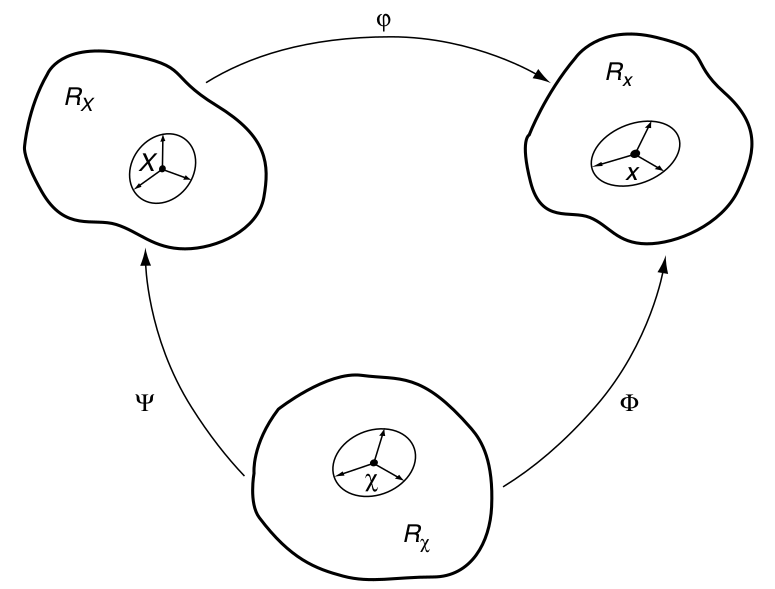
\includegraphics[width=0.5\textwidth]{Domains}
    \caption{The motion the body in the ALE formulation. The axes $\chi, \mathbf{X}$ and $\mathbf{x}$ represent the Eulerian frame in the body. While the $\mathbf{R}_{\chi}, \mathbf{R}_{\mathbf{X}}$ and $\mathbf{R}_{\mathbf{x}}$ represent the Lagrangian domain. The Final state of the body is represented by $\mathbf{R}_{\mathbf{x}}, \mathbf{x}$, which can be obtained by Lagrangian transformation $\Psi$ with respect to fixed system $\mathbf{R}_{\chi}, \chi$ and then Eulerian transformation $\varphi$ with respect to $\mathbf{R}_{\mathbf{X}}, \mathbf{X}$.}
    \label{fig:ALEdomain}
\end{figure}

\section{Vehicle Model}
\subsection{Model Assumption}
\label{sec:ALEModelAssumption}
For the model presented herein, the following assumptions are made (to address some performance issues arising if a full multi-body-dynamic formulation is used).
\begin{enumerate}
    \item There are no torsional springs between the wheels and the main body.
    \item The wheels and tyres are constrained to be vertically below the corner of the main body at all times.
    \item The moment of inertia of the main body remains constant which implies the angles of rotation for the centre of gravity are small.
\end{enumerate}
The aforementioned assumptions result in a formulation where the horizontal motion of the vehicle is independent of the vertical motion while the vertical motion is still impacted due to the rotational components arising from the horizontal force. The resulting physical system is shown in figure \ref{fig:ALEstick}. 
\begin{figure}[!ht]
    \centering
    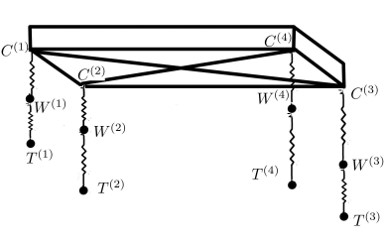
\includegraphics[width=0.45\textwidth]{ALE_stick_diagram}
    \caption{Resulting Physical system with the assumptions taken in account for ALE modelling.}
    \label{fig:ALEstick}
\end{figure}

\noindent An illustrative example of Lagrangian-Eulerian frame is given by the circular motion of the vehicle, represented in \Fref{fig:Eg_Lagrangian_Eulerian_Circular}. As well, by this figure we introduce the notations for $x$, $y$ and $z$ axes, the $z$ axis being oriented downwards with respect to centre of mass and the main motion of the vehicle in the $X-Y$ plane. 
%TODO: change figure to match coosy standards

\begin{figure}[!ht]
    \centering
    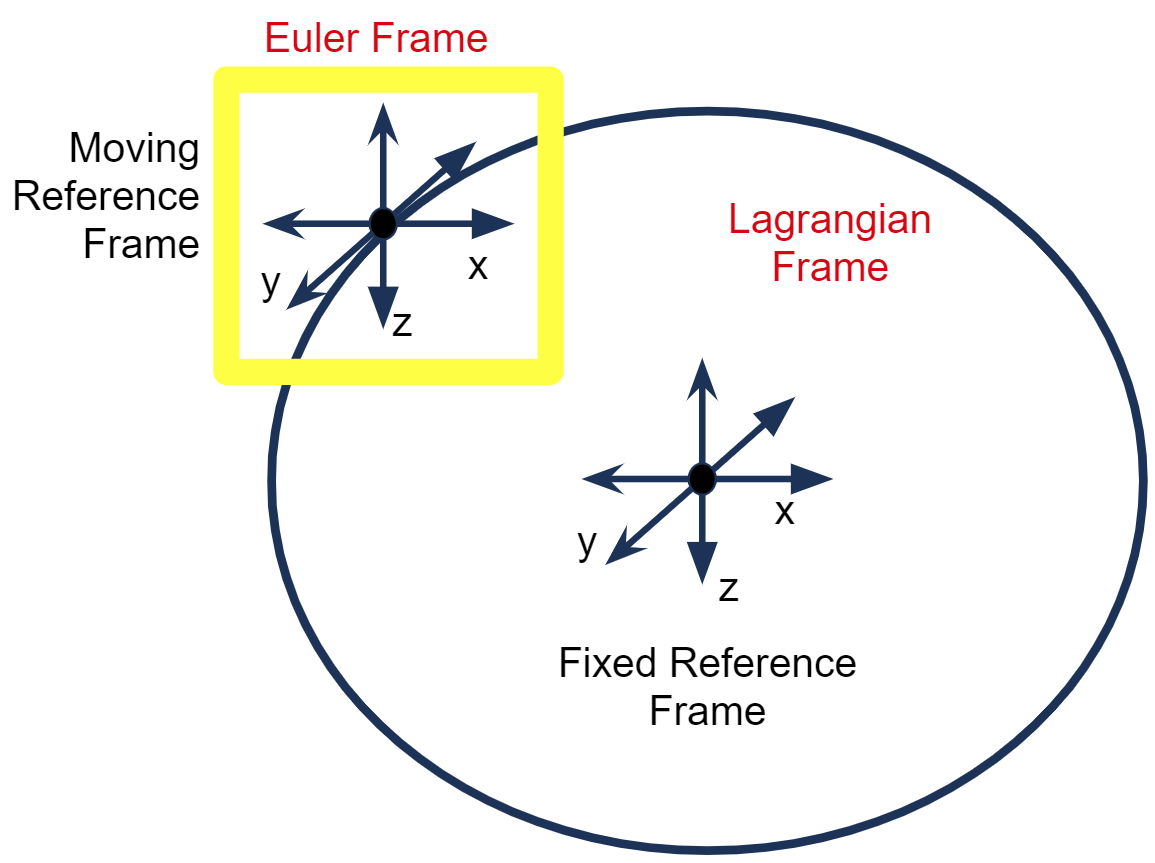
\includegraphics[width=0.45\textwidth]{Eg_Lagrangian_Eulerian_Circular}
    \caption{Example of Lagrangian-Eulerian frame for uniform circular motion}
    \label{fig:Eg_Lagrangian_Eulerian_Circular}
\end{figure}

\subsection{Model Formulation}
\label{subsection:ALEModelFormulation}
The considerations made in section \ref{sec:ALEModelAssumption} allow for a reduction in translational degrees of freedom along the $X-Y$ axes to two, which are the $X-Y$ coordinates of the centre of gravity of the main body. Additionally, the overall rotational degree of freedom is also reduced along the $Z$ axis to one, being the rotation of the main body. The coordinates of the other eight components can be evaluated by the constraint equations. The resulting simplified system was used as the Lagrangian domain. Since the horizontal motion of the body is not affected by the vertical motion, the Lagrangian frame was constrained to move in the $X-Y$ plane. This results in a reduced system having only three degrees of freedom describing the Lagrangian state of the vehicle, and can be written in the following form. \par
\begin{equation}
     \mathbf{R}_{\phi} = \begin{pmatrix} 
                        X_{\phi} \\
                        Y_{\phi} \\
                        \theta_{\phi}
                        \end{pmatrix},
\end{equation}
where:
\begin{itemize}
    \item $\mathbf{R}_{\phi}$: State vector of Lagrangian Domain.
    \item $X_{\phi}$: $X$ coordinate of the Centre of Gravity of the main body.
    \item $Y_{\phi}$: $Y$ coordinate of the Centre of Gravity of the main body.
    \item $\theta_{\phi}$: Angle along $Z$ axis for the Centre of Gravity of main body.
\end{itemize}


\noindent In contrast to the Lagrangian domain, the Eulerian domain requires the solving at all the grid points constructing the Eulerian domain. Since the model is formulated such that the motion of vehicle in $X-Y$ direction can be described entirely by the motion of Lagrangian domain, the Eulerian frame is formulated such that only the translational motion along $Z$ and rotational motion along $X-Y$ axes are considered. The Eulerian Frame considers the vehicle with unexcited spring as the computational grid points and computes the transformation of these grid points. For the above described model there are eleven computational grid points, nine of which belong to the $Z$ translational motion and two belong to $X-Y$ rotational motion. Hence the Eulerian domain can be described as follows.

\begin{equation}
     \phi = \begin{pmatrix} 
                        Z_{CG}, 
                        \theta_{X},
                        \theta_{Y},
                        Z_{W1},
                        Z_{T1},
                        Z_{W2},
                        Z_{T2},
                        Z_{W3},
                        Z_{T3},
                        Z_{W4},
                        Z_{T4}
                        \end{pmatrix}^{T},
\end{equation}
where: 
\begin{itemize}
    \item $\phi$: State vector of Eulerian Domain.
    \item $Z_{CG}$: $Z$ coordinate of the Centre of Gravity of the main body.
    \item $\theta_{X}$: Angle along $X$ axis for the Centre of Gravity of main body.
    \item $\theta_{Y}$: Angle along $Y$ axis for the Centre of Gravity of main body.
    \item $Z_{Wi}$: $Z$ coordinate of the wheel i.
    \item $Z_{Ti}$: $Z$ coordinate of the tyre i.
\end{itemize}

\noindent To simulate the motion of the vehicle, the above formulated Lagrangian and Eulerian domains were solved. The position update formulation for Lagrangian domain is described in section \ref{subsection:lagrange} and for Eulerian domain in section \ref{subsection:euler}. In order to generalise the formulation, it was assumed that the vehicle is exposed to a 3D force field $\mathbf{F(x, y, z)}$. The force field $\mathbf{F}$ can come from the road or an external force field. In order to incorporate the fundamental effect of road forces, the road profiles were formulated which act as a lookup table for the force field for each kind of domain; these are described in sections \ref{par:lagrangeprofile} and \ref{par:EulerianRoad}.


\subsection{Lagrangian Domain} \label{subsection:lagrange}
In order to formulate the position update scheme for the Lagrangian domain, it is sufficient to consider the $X-Y$ components of the force acting on the vehicle. In addition to this, the motion of the Lagrangian domain formulated in section \ref{subsection:ALEModelFormulation} is equivalent to considering the motion of a rigid body in a two dimensional space. The centre of gravity of the main body of the vehicle was considered as the moving mass. Therefore the resulting system of equation is as in \eqref{eq:lagrangeframe}:
\begin{equation}
    \label{eq:lagrangeframe}
   \ddot{\mathbf{R}}_{\phi} = \mathbf{M}^{-1} \cdot \mathbf{F(x,y, \theta)}, \hspace{0.5 cm} \mathbf{F(x,y)} \in \mathbb{R}^{3},
\end{equation}
where: 
\begin{itemize}
    \item $\ddot{\mathbf{R}}_{\phi}$: Second derivative of Lagrangian state vector.
    \item $\mathbf{M}$: Cumulative mass matrix
    \item $\mathbf{F(x,y, \theta)}$: $\mathbf{x}$, $\mathbf{y}$ and $\theta$ components of force $\mathbf{F}$
\end{itemize}

\noindent Since the resulting system is a second order ODE, Störmer–Verlet method \cite{verlet1967} was employed for time integration. The updated state vector was used with the constraint equations to compute the $(x, y)$ position of each component of the vehicle.

\paragraph{Lagrange Road Profile}\label{par:lagrangeprofile}
The Lagrange Road Profile provides a proxy for the force field in $X-Y$ plane. This module acts as a lookup table and provides the force field to the Lagrangian domain. To simulate a realistic scenario the force was modelled as a function of position and time in the lookup table. 
%TODO: add appendix?
%A more detailed description on generation of road profile lookup table is provided in the Appendix \ref{Appendix:LagrangianRoadProfile}.

\subsection{Eulerian Frame} \label{subsection:euler}
A model sketch is given in \Fref{fig:model}. 
The coordinate system for the Eulerian frame is centered at the center of gravity (CoG) and the orientation follows the vehicle model standard, the $x$-axis points in the direction of forward movement and the $z$-axis points upwards. 
As already described in section \ref{subsection:ALEModelFormulation}, the behavior in the Eulerian frame is described by 11 degrees of freedom, collected in the vector $\phi$. In \Fref{fig:model}, they are enumerated as $q_1$ to $q_{11}$ (side note: since $q$ is usually used to describe a minimal set of DoFs in structural dynamics).
\begin{figure}
	\centering
	\input{formulation/fig/model.pdf_tex}
	\caption{Model sketch}
	\label{fig:model}
\end{figure}

To keep the \Fref{fig:model} from getting overcrowded, only springs and masses are depicted. 
However, in the implemented model for every spring there is also a (generally nonlinear) damper.
Wheels and wheelcarrier are represented by a (generally nonlinear) mass-spring-damper system. Each wheel is connected to a tire, which is (again) represented by a mass-spring-damper system (note: the bottom mass, belonging to tires, can be ignored if a Dirichlet boundary condition is applied to it, the boundary condition (force) can instead be applied directly to the spring, see \cite{mitschke2014}, section 2.2.2).

\paragraph{EOM}
%The Force formulation described in section  \ref{subsection:ALEModelFormulation} requires an implicit numerical scheme in the Eulerian frame. 
The equations of motion (EOM) for the Eulerian domain are derived from the force formulation in section \ref{subsection:ALEModelFormulation}.
Following is the resulting system \eqref{eq:EOMeuler}, that was comprehensively studied in \cite{sicklingerthesis}:
\begin{equation} \label{eq:EOMeuler}
     \boldsymbol{M} \ddot{\boldsymbol{\phi}}^{n+1}+ \boldsymbol{D} \dot{\boldsymbol{\phi}}^{n+1} + \boldsymbol{K}\boldsymbol{\phi}^{n+1}=\boldsymbol{f}^{n+1}
\end{equation}
where:
    \begin{itemize}
        \item $\boldsymbol{M}$ - Mass / Moment of Inertia matrix
        \item $\boldsymbol{D}$ - Damping Matrix
        \item $\boldsymbol{K}$ - Stiffness Matrix
        \item $\boldsymbol{\phi}$ - Eulerian state vector
        \item $\boldsymbol{f}$ - Force field in the Eulerian frame, see \ref{par:CoupleEulerLagrange} for $\boldsymbol{f}^{n+1}$
    \end{itemize}

\paragraph{Time integration}
Backward Euler time integration is used for the numerical time integration (just one simple choice). It is the most basic implicit time stepping method and described by the approximations of velocity and acceleration for the next time step
\begin{align}
	\dot{\boldsymbol{\phi}} &= \frac{1}{h}(\boldsymbol{\phi}^{n+1} - \boldsymbol{\phi}^n )  \label{eq:bevel} \\ 
	\ddot{\boldsymbol{\phi}} &= \frac{1}{h^2}(\boldsymbol{\phi}^{n+1} - 2\boldsymbol{\phi}^n + \boldsymbol{\phi}^{n-1}),\label{eq:beacc}
\end{align}
where $h$ is the time step size (side note: since it is an implicit time integration method, it is unconditionally stable, i.e. only the correctness of the method depends on the choice of $h$, not the stability).
Inserting the two approximations into \eqref{eq:EOMeuler} the following system of equations has to be solved for $\boldsymbol{\phi}^{n+1}$ at each time step
\begin{equation}\label{eq:beequation}
	(\frac{1}{h^2} \boldsymbol{M} + \frac{1}{h}\boldsymbol{D} + \boldsymbol{K}) \boldsymbol{\phi}^{n+1} = (\frac{2}{h^2}\boldsymbol{M} + \frac{1}{h}\boldsymbol{D}) \boldsymbol{\phi}^{n} - \frac{1}{h^2}\boldsymbol{M} \boldsymbol{\phi}^{n-1} + \boldsymbol{f}.
\end{equation}


\paragraph{Newton algorithm}
In general, equation \eqref{eq:EOMeuler} cannot be solved directly, for example due to a coupling to the Lagrangian domain, see paragraph \ref{par:CoupleEulerLagrange}, or due to nonlinear springs and dampers, see paragraph \ref{par:NonlinearSpring}. 
Therefore, Newton's method is introduced with 
\begin{equation}\label{eq:residual}
     \boldsymbol{r}(\boldsymbol{\phi}^{n+1}) = \boldsymbol{M} \ddot{\boldsymbol{\phi}}^{n+1}+ \boldsymbol{D} \dot{\boldsymbol{\phi}}^{n+1} + \boldsymbol{K}\boldsymbol{\phi}^{n+1}-\boldsymbol{f}^{n+1}\overset{!}{=}0
\end{equation}
where $\boldsymbol{r}(\boldsymbol{\phi}^{n+1})$ is the residual for the root finding problem.  
The solution is calculated iteratively via the update steps:
\begin{equation}
\boldsymbol{\phi}^{n+1}_{new} = \boldsymbol{\phi}^{n+1}_{old} - \boldsymbol{J}^{-1}\boldsymbol{r}(\boldsymbol{\phi}^{n+1}_{old}),
\end{equation}
where $\boldsymbol{J}$ is the Jacobian of $\boldsymbol{r}(\boldsymbol{\phi}^{n+1}_{old})$. The Jacobian can be described analytically as:
\begin{equation}
    \label{eq:constantjacobian}
    \boldsymbol{J} = \frac{d\boldsymbol{r}}{d\boldsymbol{\phi}^{n+1}} =  \boldsymbol{M} \frac{d \ddot{\boldsymbol{\phi}}^{n+1}}{d \boldsymbol{\phi}^{n+1}} +  \boldsymbol{D} \frac{d \dot{\boldsymbol{\phi}}^{n+1}}{d \boldsymbol{\phi}^{n+1}} + \boldsymbol{K}  - \frac{d \boldsymbol{f}^{n+1}}{d \boldsymbol{\phi}^{n+1}}.
\end{equation}
The first and second derivatives of $\boldsymbol{\phi}^{n+1}$ depend on the time stepping scheme. Here the damping $\boldsymbol{D}$ and stiffness $\boldsymbol{K}$ are assumed to be constant. The only unknown in equation \eqref{eq:constantjacobian} is the derivative of the force, which depends on the boundary conditions and is specified in section \ref{par:EulerianRoad} more thoroughly.
Starting from the time discretized EOMs in \eqref{eq:beequation}, the same residual and Jacobi matrix are obtained if the BE formulations \eqref{eq:bevel},\eqref{eq:beacc} are inserted into the equations \eqref{eq:constantjacobian},\eqref{eq:residual} presented herein
(side note: the Newton algorithm can also be applied to the linear system of equations. Instead of solving the system directly, one iteration of the Newton algorithm is carried out, which leads to a system of equations of the same size to be solved for the update $\delta = \boldsymbol{J}^{-1}\boldsymbol{r}$).

\paragraph{Stabilizer bar}
In the front and in the back, seen in \Fref{fig:model}, there is a stabilizer bar connecting the left and right hand side. The stabilizer bars can be described by the force equations $F_l$ and $F_r$ on the left and right hand side
\begin{align}
	F_l &= k_\mathrm{stab} \cdot (q_r - q_l)\\
	F_r &= k_\mathrm{stab} \cdot (q_l - q_r)	
\end{align}
which depend on the difference of the displacements on the left $q_l$ (positive $y$-direction) and right $q_r$ (negative $y$-direction) hand sides.
The forces are acting in positive $z$-direction, s.t. the stabilizer bar is in equilibrium. 
The stabilizer bar is used to control lateral dynamics ("Querdynamik") since it results in a force on the wheel on one side if the vertical displacement of the other wheel is different. 
In simpler words, the stabilizer bar pulls the wheel on the other side behind.
For more information, see \cite{mitschke2014} (section 15.5).


\paragraph{State Dependent Stiffness and Damping Coefficients}\label{par:NonlinearSpring}
In terms of physical correctness, the feature to provide lookup tables for stiffness and damping for the springs between body and wheel (and between wheel and tire) was introduced. Those lookup tables correspond to experimentally determined data, which can not be described by an analytical function. The given values get interpolated according to the current spring lengths. This introduces position-dependent $\boldsymbol{D}$ and $\boldsymbol{K}$ matrices.
\begin{equation}\label{eq:EOMnonlin}
	\boldsymbol{M} \ddot{\boldsymbol{\phi}}^{n+1}+ \boldsymbol{D}^{n+1} \dot{\boldsymbol{\phi}}^{n+1} + \boldsymbol{K}^{n+1}\boldsymbol{\phi}^{n+1}=\boldsymbol{f}^{n+1}
\end{equation}
The corresponding Jacobian can not be determined fully analytically, as the derivative of $\boldsymbol{D}$ and $\boldsymbol{K}$ depends on the derivative of the according lookup table, which is unknown and has to be computed during runtime. This derivative also depends on the type of interpolation. The interpolation can be done linearly or cubic. Cubic has the benefit that not only the function itself but also the first derivative is continuous, which might lead to less Newton iterations for very stiff systems. For the sake of this project, a dummy lookup table was used, which got sampled from a quadratic function. Therefore, a linear interpolation was sufficient and was used for all conducted results.

\noindent A further challenge is the situation depending force $\boldsymbol{f}^{n+1}$ acting on the system. It can depend on the acceleration, velocity and position. Hence, the Jacobian has to be adapted according to the situation. The forces acting on the tyres are shown in the following chapter. The total Jacobian can be described as:
\begin{equation}\label{eq:JacobiNonlin}
	\boldsymbol{J} = \boldsymbol{M} 
	\frac{d \ddot{\boldsymbol{\phi}}^{n+1}}{d \boldsymbol{\phi}^{n+1}} 
	+ \frac{d \boldsymbol{D}^{n+1}}{d \boldsymbol{\phi}^{n+1}} \dot{\boldsymbol{\phi}}^{n+1} + \boldsymbol{D}^{n+1} \frac{d \dot{\boldsymbol{\phi}}^{n+1}}{d \boldsymbol{\phi}^{n+1}} + \frac{d \boldsymbol{K}^{n+1}}{d \boldsymbol{\phi}^{n+1}} \boldsymbol{\phi}^{n+1} + \boldsymbol{K}^{n+1}  - \frac{d \boldsymbol{f}^{n+1}}{d \boldsymbol{\phi}^{n+1}}
\end{equation}

\paragraph{State Dependent Stiffness and Damping Forces} \label{par:NonlinearSpringForce}
However, there is also the case when the lookup tables do not provide stiffness and damping parameters but forces, depending on the relative displacements and velocities. Now there are two possibilities to incorporate them into the framework established so far:
\begin{enumerate}
	\item Compute the stiffness and damping coefficients from the lookup tables and stick with \eqref{eq:EOMnonlin}, \eqref{eq:JacobiNonlin}.
	\item Use the forces directly by amending the matrix-vector formulation in \eqref{eq:EOMeuler}.
\end{enumerate}
Both ways work, have their pros and cons and will be sketched quickly, neglecting the dampers for brevity. 

The main problem of the first method is the computation of the coefficients from the forces. In general the forces of the springs are nonlinear and depend on the stiffness of the spring, which herein is state dependent itself.
\begin{equation}
	F_k = f(k(\phi),\phi)
\end{equation}
For the linear case, it is well known that the spring force reduces to
\begin{equation}\label{eq:SpringForceLinear}
	F=k\cdot\triangle l(\phi),
\end{equation}  
where $\triangle l(\phi)$ is the change in the length of the spring. 
For this case, the stiffness coefficients can be easily computed from the given lookup tables. 
However, this is not the case for the nonlinear case which will be shown with a small example, sketched in \Fref{fig:nonlinspring} with the lookup table given in \Fref{tab:lookup1}. 

\begin{figure}
	\centering
	%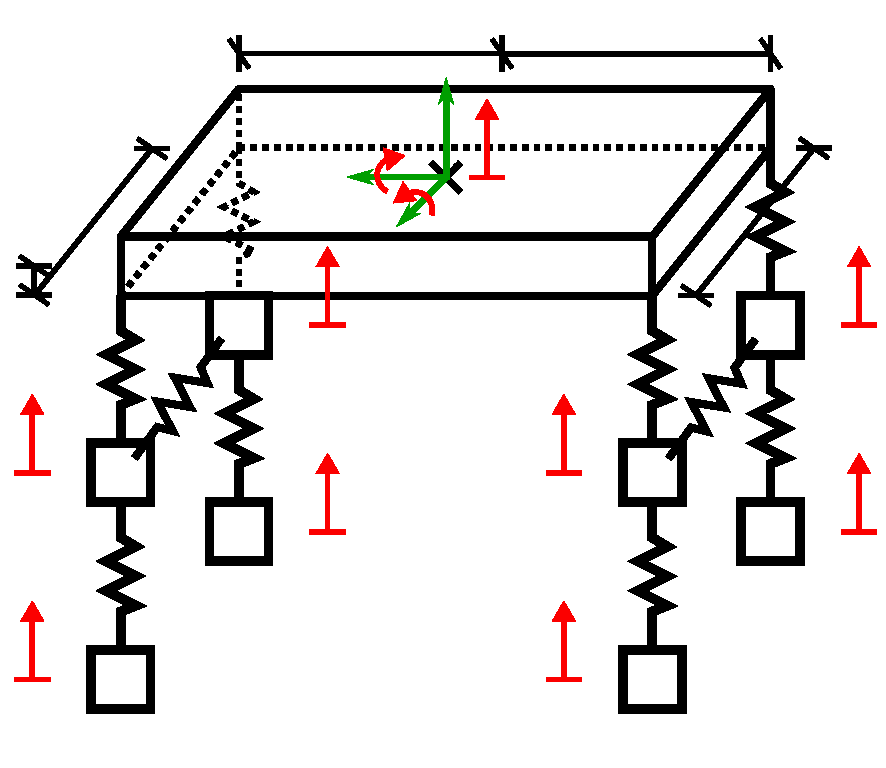
\includegraphics[width=0.9\textwidth]{model.pdf}
	\input{formulation/fig/nonlinspring.pdf_tex}
	\caption{Problem for nonlinear spring example}
	\label{fig:nonlinspring}
\end{figure}
\begin{table}
	\caption{Lookup table for nonlinear spring example in \Fref{fig:nonlinspring}}
	\begin{tabular}{lccccc}
		\toprule
		$\triangle l$ & -0.1 & 0 & 0.1 & 0.2 & 0.3\\
		$F$ & -0.3 & 0 & 0.3 & 0.5 & 0.9 \\
		\bottomrule
	\end{tabular}
	\label{tab:lookup1}
\end{table}

For the static case, the external force $F$ has to equal the spring force $F(k,\triangle l)$ and since the problem is one dimensional, the relative length of the spring $\triangle l$ is entirely described by the  displacement $u$ and the solution  can be easily read from the plot in \Fref{fig:nonlinspring}. 
Linear interpolation is assumed between the points given in the lookup table, resulting in three different linear equations for the three sections in the plot
\begin{align*}
	F_1 &= 3 u &u \epsilon [-0.1,0.1],\\
	F_2 &= 2 u + 0.1 & u \epsilon [0.1,0.2],\\
	F_3 &= 4 u - 0.3, & u \epsilon [0.2,0.3]. 
\end{align*}
It is easy to see that even if the stiffness coefficient is computed as slope from the lookup table, the (nonlinear) history has to be considered as well or otherwise the external force $F = 0.4$ would give a solution $u = \nicefrac{F}{k} = \nicefrac{0.4}{2} = 0.2 \neq 0.15$. It is easy to see that forcing the system, where the forces are nonlinear, to fit into the linear description used to build the stiffness matrix, requires extra effort. 
Having said this, assuming linear interpolation (and with little extra effort also other interpolations can be used), it only requires adding the constants to the residuum and the Jacobian stays the same, since the derivative of the additional constants vanish.
The problem of the first method leads to the second method, complemented by the observation that after computing the stiffness coefficients, the stiffness matrix is multiplied by the state vector in \eqref{eq:EOMeuler}, which gives the forces.

The disadvantage of this second method is that the formulation of the EOMs \eqref{eq:EOMeuler} is replaced by the more general
\begin{equation}\label{eq:EOMnonlinForce}
	     \boldsymbol{M} \ddot{\boldsymbol{\phi}}^{n+1}+ \boldsymbol{F_d} (\dot{\boldsymbol{\phi}}^{n+1})  + \boldsymbol{F_k}(\boldsymbol{\phi}^{n+1})=\boldsymbol{f}^{n+1}
\end{equation} 
which is less common and (therefore) less intuitive.
There are different ways to derive the EOMs \eqref{eq:EOMeuler}, one of which is using Newton's second law, the conservation of momentum ("Impulserhaltungssatz"), which states that external forces equal internal forces or $m\ddot{q} = \sum F$. 
Conservation of momentum holds for each of the nine masses in the Eulerian model \Fref{fig:model}. 
The car body also has two rotational DoFs for which the equations are formulated similarly (just with inertias instead of masses and moments instead of forces: $I\ddot{\varphi} = \sum M$). 
Using the linear formulation for the forces \eqref{eq:SpringForceLinear}, the stiffness matrix is built.
For nonlinear forces this last step is skipped and instead of stiffness matrix times displacement, the equation contains the 11-dimensional vector, which obviously also contains all the model information the stiffness matrix does. 
For the model in \Fref{fig:model} it reads
\begin{equation}\label{eq:ForceModel}
	\boldsymbol{F_k} = 
	\begin{bmatrix}
		f_1 + f_3 + f_5 + f_7 \\
		f_1 \cdot l_\mathrm{lat,f} - f_3 \cdot l_\mathrm{lat,f} + f_5 \cdot l_\mathrm{lat,r} -  f_7 \cdot l_\mathrm{lat,r} \\
		-f_1 \cdot l_\mathrm{long,f} - f_3 \cdot l_\mathrm{long,f} + f_5 \cdot l_\mathrm{long,r} + f_7 \cdot l_\mathrm{long,r} \\
		-f_1 + f_2 \\
		-f_2 \\
		-f_3 + f_4 \\
		-f_4 \\
		-f_5 + f_6 \\
		-f_6 \\
		-f_7 + f_8 \\
		-f_8 \\
	\end{bmatrix}
\end{equation}
To solve the nonlinear equation \eqref{eq:EOMnonlinForce}, the Newton iteration is used again with residual
\begin{equation}
   \boldsymbol{r}(\boldsymbol{\phi}^{n+1}) = \boldsymbol{M} \ddot{\boldsymbol{\phi}}^{n+1}+ \boldsymbol{F_d} (\dot{\boldsymbol{\phi}}^{n+1})  + \boldsymbol{F_k}(\boldsymbol{\phi}^{n+1}) - \boldsymbol{f}^{n+1} \overset{!}{=}0
\end{equation}
and Jacobian
\begin{equation}\label{eq:JacobiNonlinForce}
	\boldsymbol{J} = \frac{d\boldsymbol{r}}{d\boldsymbol{\phi}^{n+1}} = M \frac{d \ddot{\boldsymbol{\phi}}^{n+1}}{d \boldsymbol{\phi}^{n+1}} + \frac{d \boldsymbol{F_d}(\dot{\boldsymbol{\phi}}^{n+1})}{d \dot{\boldsymbol{\phi}}^{n+1}}\frac{d \dot{\boldsymbol{\phi}}^{n+1}}{d 
	\boldsymbol{\phi}^{n+1}} + \frac{d \boldsymbol{F_k}(\boldsymbol{\phi}^{n+1})}{d \boldsymbol{\phi}^{n+1}} -  \frac{d \boldsymbol{f}^{n+1}}{d \boldsymbol{\phi}^{n+1}}
\end{equation}
Using the premise of this paragraph that the nonlinear force is obtained from lookup tables where it depends on the relative displacement / change in length of the springs gives
\begin{equation}\label{eq:ForceDeriv}
	\frac{d \boldsymbol{F_k}(\boldsymbol{\phi}^{n+1})}{d \boldsymbol{\phi}^{n+1}} = \frac{\partial \boldsymbol{F_k}}{\partial \triangle\boldsymbol{l}} \frac{\partial \triangle\boldsymbol{l}}{\partial \boldsymbol{\phi}^{n+1}}.
\end{equation}
where the relative lengths of the springs are obtained analytically as
\begin{equation}
	\triangle \boldsymbol{l} (\boldsymbol{\phi}) = 
	\begin{bmatrix}
		q_1 + l_\mathrm{lat,f}\cdot q_2 - l_\mathrm{long,f}\cdot q_3 - l_\mathrm{cog,spring} - q_4 \\
		q_4 - q_5 \\
		q_1 - l_\mathrm{lat,f}\cdot q_2 - l_\mathrm{long,f}\cdot q_3 - l_\mathrm{cog,spring} - q_6 \\
		q_6 - q_7 \\
		q_1 + l_\mathrm{lat,r}\cdot q_2 + l_\mathrm{long,r}\cdot q_3 - l_\mathrm{cog,spring} - q_8 \\
		q_8 - q_9 \\
		q_1 - l_\mathrm{lat,r}\cdot q_2 + l_\mathrm{long,r}\cdot q_3 - l_\mathrm{cog,spring} - q_{10} \\
		q_{10} - q_{11}
	\end{bmatrix}
\end{equation}
where the rotation matrix with the small angle approximation of \fref{sec:ALEModelAssumption} is used to compute the position of the four corners of the body (where the mass-spring-damper model of the wheels/wheel carriers are attached).
\begin{equation}
	R = R_y(q_3) \cdot R_x (q_2) = 
	\begin{bmatrix}
		\cos q_3 & \sin q_3 \sin q_2 & \sin q_3 \cos q_2 \\
		0 & \cos q_2 & -\sin q_2 \\ 
		-\sin q_3 & \cos q_3 \sin q_2 & \cos q_3 \cos q_2
	\end{bmatrix} \approx 
	\begin{bmatrix}
		1 & 0 & q_3 \\
		0 & 1 & -q_2 \\
		-q_3 & q_2 & 1 
	\end{bmatrix}
\end{equation}

Some notes:
\begin{itemize}
	\item Both the function $\boldsymbol{F_k}$ as well as the derivative in the Jacobian can be computed analytically beforehand, see \eqref{eq:ForceModel}.
	\item Technically, the vector $\boldsymbol{F_k}$ in \eqref{eq:ForceModel} depends on the 8 forces of the different springs  $\boldsymbol{f_k} = [f_1(\triangle l_1),\\ f_2(\triangle l_2), ..., f_8(\triangle l_8)]^\mathrm{T}$ and the derivative for the force w.r.t. the relative lengths is $\nicefrac{\partial \boldsymbol{F_k}}{\partial \boldsymbol{f_k}}\nicefrac{\partial \boldsymbol{f_k}}{\partial \triangle\boldsymbol{l}}$, where the second derivative depends on the interpolation in the lookup table. 
	\item At runtime, only the values of the forces corresponding to the state values $\boldsymbol{\phi}^{n+1}$ have to be obtained (by interpolation) from the lookup table.
	\item In the code, two different interpolation types are provided, linear interpolation (which is also used in Abaqus) and a spline interpolation (which is more physical, since continuous and therefore should lead to improved convergence).  
	\item The backward euler time integration is integrated into the algorithm as before, using the approximations for acceleration \eqref{eq:beacc} and velocity \eqref{eq:bevel}.
	\item The damping force and its derivative in the Jacobian \eqref{eq:JacobiNonlinForce} can be obtained with the same functions as for the spring force, using the velocity \eqref{eq:bevel} instead of the displacement, and of course the lookup table for the damping forces and relative velocities. Only difference in the Jacobian is the last term $\nicefrac{d \dot{\boldsymbol{\phi}}^{n+1}}{d \boldsymbol{\phi}^{n+1}}$ which is a scalar computed according to the time integration scheme used.
	\item A word on dimension: In \eqref{eq:ForceDeriv}, the force $\boldsymbol{F_k}$ is a 11x1 vector and $\triangle\boldsymbol{l}$ is an 8x1 vector, which gives an 11x8 matrix with partial derivatives. Since $\boldsymbol{\phi}^{n+1}$ is (obviously) 11x1, the second derivative matrix is 8x11 and the multiplication gives the expected 11x11 for the Jacobian.
\end{itemize}


\paragraph{Coupling to Lagrangian domain}\label{par:CoupleEulerLagrange}
Since the force field in the Eulerian frame has a component which couples it to the state of Lagrangian frame as well as the force acting on the Lagrangian domain, the term $\boldsymbol{f}^{n+1}$ combines the contribution coming from the Lagrangian frame in the form of Torque and $F(z)$. The Torque from the Lagrangian frame is computed by summing up the contribution from the inertial forces and the pseudo-forces (if the Eulerian frame is non-inertial). Hence the resulting $\boldsymbol{f}^{n+1}$ has the form
\begin{align}
	\boldsymbol{f}^{n+1} &= \begin{pmatrix} 
		\mathbf{F(z_{CG})}\\
		\mathbf{T(x_{CG})}\\
		\mathbf{T(y_{CG})}\\
		\mathbf{F(z_{W1})}\\
		\mathbf{F(z_{T1})}\\
		\mathbf{F(z_{W2})}\\
		\mathbf{F(z_{T2})}\\
		\mathbf{F(z_{W3})}\\
		\mathbf{F(z_{T3})}\\
		\mathbf{F(z_{W4})}\\
		\mathbf{F(z_{T4})}
	\end{pmatrix} + 
	\begin{pmatrix} 
		0\\
		\mathbf{T_{proj_{x}}}\\
		\mathbf{T_{proj_{y}}}\\
		0\\
		0\\
		0\\
		0\\
		0\\
		0\\
		0\\
		0\\
	\end{pmatrix} \\ \intertext{where:}
	\mathbf{T_{proj}} &= \boldsymbol{\Psi}(t, \mathbf{R}_{\phi})
	\label{eq:f_Eulerian}
\end{align}
and $\boldsymbol{\Psi}$ is the projection operator.

\paragraph{Boundary conditions}
The boundary conditions mentioned so far are external forces $\boldsymbol{f}^{n+1}$ in the EOMs \eqref{eq:EOMeuler}, \eqref{eq:EOMnonlin}, \eqref{eq:EOMnonlinForce}.
Furthermore, there exist Dirichlet boundary conditions, where the value of the quantity of interest (here: displacements and rotations) is prescribed on the boundary (for the sake of completeness, there also exist Neumann boundary conditions where the derivative of the quantity of interest is given on the boundary (especially for fluid- and thermodynamics), as well as Robin boundary conditions where the two are mixed).

\paragraph{Eulerian Road Profiles} \label{par:EulerianRoad}
\noindent The Eulerian road profiles provide a lookup proxy method similar to that described in section \ref{par:lagrangeprofile}. This method generates a time and state dependent force field lookup table which is used during the computation of the Eulerian state. The following subsections describe some Eulerian road profiles.

\paragraph{Flat Road} \label{par:FlatRoad}
The next more complicated profile is for a completely flat road. The constraint for a flat road is non moving tyres in z-direction. This can be enforced by setting the acceleration of the tyres to 0, which results in
\begin{align}
    \boldsymbol{f}^{n+1}_{tyre} &=  \left(\boldsymbol{D}^{n+1} \dot{\boldsymbol{\phi}}^{n+1} + \boldsymbol{K}^{n+1}\boldsymbol{\phi}^{n+1}\right)_{tyre}
\end{align}
for the force and in
\begin{equation}
     \boldsymbol{J}(\boldsymbol{\phi}^{n+1})_{tyre} = \left(\boldsymbol{M} \frac{d \ddot{\boldsymbol{\phi}}^{n+1}}{d \boldsymbol{\phi}^{n+1}}\right)_{tyre}
\end{equation}
for the Jacobian.

\paragraph{Homogeneous Dirichlet boundary condition}
A homogeneous Dirichlet boundary condition on the tires means the nodes are fixed. There are (mainly) two possibilities to incorporate this into the EOMs.
\begin{enumerate}
	\item Delete the rows and columns associated with the dof.
	\item Zero out the rows and columns associated with the dof, replacing the entry of the main diagonal of the system matrix by 1, s.t. the equation for the dof reads: $1 u^{n+1} = 0$. 
\end{enumerate}
Advantage of the first possibility is that the dimension of the system of equations is reduced by the number of fixed dofs, while using the second method has the advantage that it is easier to debug the code since it is more obvious to spot errors in the equations, e.g. during assembly or differentiation.
(Note 1: The boundary conditions have to be applied to the Jacobian as well. Note 2: Both methods can be applied to the formulation with the nonlinear forces \eqref{eq:EOMnonlinForce}. The functions have to be changed for the first, entries in the force vectors zeroed for the second.)

\paragraph{Bumpy road}
A nonhomogeneous Dirichlet boundary condition on the tires means the displacement is prescribed, but not necessarily zero, which makes it an extension to the homogeneous Dirichlet boundary condition.
A lookup table provides a displacement corresponding to a certain time  for each of the tires. 
The values for each time step are interpolated from the lookup table.
The displacements on the tires result in an additional force in \eqref{eq:beequation} (which of course is zero for the homogeneous boundary condition, since the displacement is zero)
\begin{equation}
	\boldsymbol{f}^{n+1}_\mathrm{tire} = -(\frac{1}{h^2} \boldsymbol{M} + \frac{1}{h}\boldsymbol{D} + \boldsymbol{K}) \boldsymbol{\phi}^{n+1}_\mathrm{tire}.
\end{equation}
Furthermore, the displacement can be treated with one of the methods introduced in the previous paragraph, amending the second possibility s.t. the equation reads $1 u^{n+1} = u^{n+1}_\mathrm{tire}$.


% \section{Lagrangian Frame}
% For a well defined simulation some boundary conditions regarding the road had to be introduced. Those conditions can differ from road to road. Therefore, it made sense to distinguish certain road profiles, further elaborated in the next few sections. Due to the decoupling of the Eulerian and the Lagrangian frame, described in section \ref{subsection:ModelDescription}, it made more than sense to also decouple the road profiles. Figure \ref{fig:ALE_Profiles} presents an overview of the implemented road profiles.

% \begin{figure}[!ht]
%     \centering
%     \includegraphics[width=0.5\textwidth]{pics/ALE_Profiles.PNG}
%     \caption{Overview of Road Profiles}
%     \label{fig:ALE_Profiles}
% \end{figure}

% \subsubsection{Lagrangian Profiles}
% The Lagrangian profiles describes the road path x and y direction. This profile is only used in the Lagrangian calculation part of the simulation and has no effect on the Eulerian part.
